% Preamble
\documentclass[compress,aspectratio=169]{beamer}


% Packages
\usepackage{amsmath}
\usepackage{graphicx}
\usepackage{xcolor}
\usepackage{tikz}
\usepackage{amssymb}
\usetikzlibrary{shapes, shadows, arrows,arrows.meta}
\usetikzlibrary{positioning}
\usepackage{hyperref}
\usepackage{mathtools}
% Bib
\usepackage[style=numeric-comp,natbib=true]{biblatex}
\AtEveryBibitem{%
	\clearfield{issn} % Remove issn
	\clearfield{doi} % Remove doi

	\ifentrytype{online}{}{% Remove url except for @online
		\clearfield{url}
	}
}
\addbibresource{../../references.bib}

% Setup
\def\changemargin{\list{}{\rightmargin.2\linewidth\leftmargin.2\linewidth}\item[]}
\let\endchangemargin=\endlist

% Theme
\usepackage[scaled]{helvet}
\renewcommand\familydefault{\sfdefault}
\usepackage[T1]{fontenc}

\setbeamertemplate{navigation symbols}{}
\setbeamertemplate{frametitle}{
	\vspace{.5in}
	\raggedright\insertframetitle%
}
\setbeamertemplate{bibliography item}{\insertbiblabel}
\setbeamercolor{frametitle}{fg=black}
\setbeamercolor{title}{fg=black}
\setbeamertemplate{itemize item}{\color{gray}$\blacktriangleright$}
\setbeamercolor{normal text}{fg=darkgray}
\setbeamercolor{bibliography item}{fg=gray}
\setbeamercolor{bibliography entry author}{fg=black}
\setbeamercolor{bibliography entry title}{fg=darkgray}
\setbeamercolor{bibliography entry authors}{fg=darkgray}
\setbeamercolor{bibliography entry location}{fg=gray}
\setbeamercolor{bibliography entry note}{fg=gray}
\setbeamercolor{bibliography entry journal}{fg=gray}

\definecolor{myred}{RGB}{255, 42, 42}
\definecolor{mygreen}{RGB}{113, 200, 55}
\definecolor{myblue}{RGB}{42, 127, 255}


% Meta
\title{Structured Multilinear Discriminant Analysis\\ for ERP Classification}
\author{\textbf{Arne Van Den Kerchove}, Arno Libert, \\ Hakim
	Si-Mohammed, Marc M. Van Hulle \\ \& François Cabestaing}
\institute{CORTICO 2022}
\date{}
\titlegraphic{\includegraphics{images/logo.png}}

% Document
\begin{document}

% ================================================================================
\frame{
	\vskip0pt plus 1filll
		{\usebeamerfont{title}\usebeamercolor[fg]{title}\inserttitle}
	\bigskip

	\insertauthor \bigskip

	\insertinstitute \bigskip

	\insertdate \bigskip

	\inserttitlegraphic
	\vskip0pt plus 1filll

}

% ================================================================================
%\frame{
%	\frametitle{ERPs with 64 channels of 64 time samples each\ldots}
%	
\includegraphics[height=.43\linewidth]{images/compare_information_1.eps}
%}
%\frame{
%	\frametitle{\ldots have a large number of covariance parameters\ldots}
%	\includegraphics[height=.43\linewidth]{images/compare_information_2.eps}
%}
%\frame{
%	\frametitle{\ldots but this number can be reduced.}
%	\includegraphics[height=.43\linewidth]{images/compare_information_3.eps}
%}
%
% ================================================================================
\frame{
	\frametitle{Covert attention BCIs operate in \\ the visual periphery}
	\begin{columns}[onlytextwidth]
		\begin{column}{.45\linewidth}
			\textbf{Overt} BCI operation
			\bigskip

			\centering
			\includegraphics[width=\linewidth]{images/overt.pdf}
		\end{column}%
		\begin{column}{.45\linewidth}
			\textbf{Covert} BCI operation
			\bigskip

			\centering
			\includegraphics[width=\linewidth]{images/covert.pdf}
		\end{column}
	\end{columns}
	\bigskip
	\raggedright
	\begin{flushright}
		\textcolor{mygreen}{mental attention} \\
		\textcolor{myred}{vision}
	\end{flushright}
}
% ================================================================================
\frame{
	\frametitle{ERPs are spatiotemporal data points}
	\begin{changemargin}
		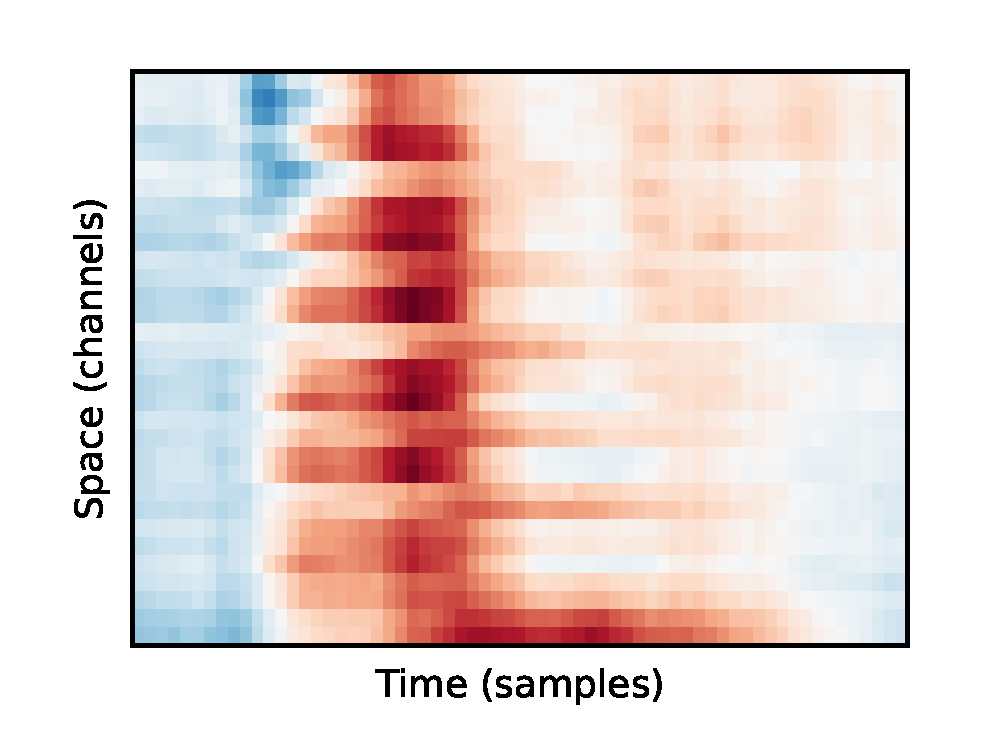
\includegraphics[width=\linewidth]{figures/grand_avg.eps}
	\end{changemargin}
}


% ================================================================================
\frame{
	\frametitle{Spatiotemporal covariance matrices are large and hard to
		invert}
	$$
		\vcenter{\hbox{\includegraphics[width=.45\linewidth]{figures/emp_cov_label.png}}}^{-1}
		=
		\vcenter{\hbox{\includegraphics[width=.45\linewidth]{figures/emp_prec_label.png}}}
	$$
}
% ================================================================================
\frame{
	\frametitle{Spatiotemporal classifiers \\ suffer from curse of
		dimensionality}

	\begin{minipage}[t]{.5\linewidth}
		\textbf{Problem:}
		\begin{itemize}
			\item Slow training
			\item High memory usage
			\item Prone to overfitting
			\item Lots of training data needed
		\end{itemize}
	\end{minipage}%
	\begin{minipage}[t]{.5\linewidth}
		\textbf{Solutions}:
		\begin{itemize}
			\item Feature selection
			\item Aggregate to single domain
			\item \textbf{Structured+regularized estimation}
		\end{itemize}

	\end{minipage}
}

% ================================================================================
\frame{
	\frametitle{Spatiotemporal covariance is decomposable \\ into stationary
		noise sources}

	\begin{minipage}{.5\linewidth}
		\begin{align*}
			\includegraphics[width=.8\linewidth]{figures/emp_cov.png}
		\end{align*}
	\end{minipage}%
	\begin{minipage}{.5\linewidth}
		\begin{align*}
			= \lambda_1 *
			\vcenter{\hbox{\includegraphics[width=.245\linewidth]{figures/sp_cov_2.png}}}
			 & \otimes
			\vcenter{\hbox{\includegraphics[width=.245\linewidth]{figures/tmp_cov_2.png}}}
			\\
			+ \lambda_2 *
			\vcenter{\hbox{\includegraphics[width=.245\linewidth]{figures/sp_cov_1.png}}}
			 & \otimes
			\vcenter{\hbox{\includegraphics[width=.245\linewidth]{figures/tmp_cov_1.png}}}
			\\
			+ \lambda_3 *
			\vcenter{\hbox{\includegraphics[width=.245\linewidth]{figures/sp_cov_3.png}}}
			 & \otimes
			\vcenter{\hbox{\includegraphics[width=.245\linewidth]{figures/tmp_cov_3.png}}}
			+ \cdots
		\end{align*}
	\end{minipage}
}

\frame{
	\frametitle{The first term suffices}

	\begin{minipage}{.5\linewidth}
		\begin{align*}
			\includegraphics[width=.8\linewidth]{figures/emp_cov.png}
		\end{align*}
	\end{minipage}%
	\begin{minipage}{.5\linewidth}
		\begin{align*}
			=
			\vcenter{\hbox{\includegraphics[width=.245\linewidth]{figures/sp_cov_2.png}}}
			 & \otimes
			\vcenter{\hbox{\includegraphics[width=.245\linewidth]{figures/tmp_cov_2.png}}}
		\end{align*}
		\centering
		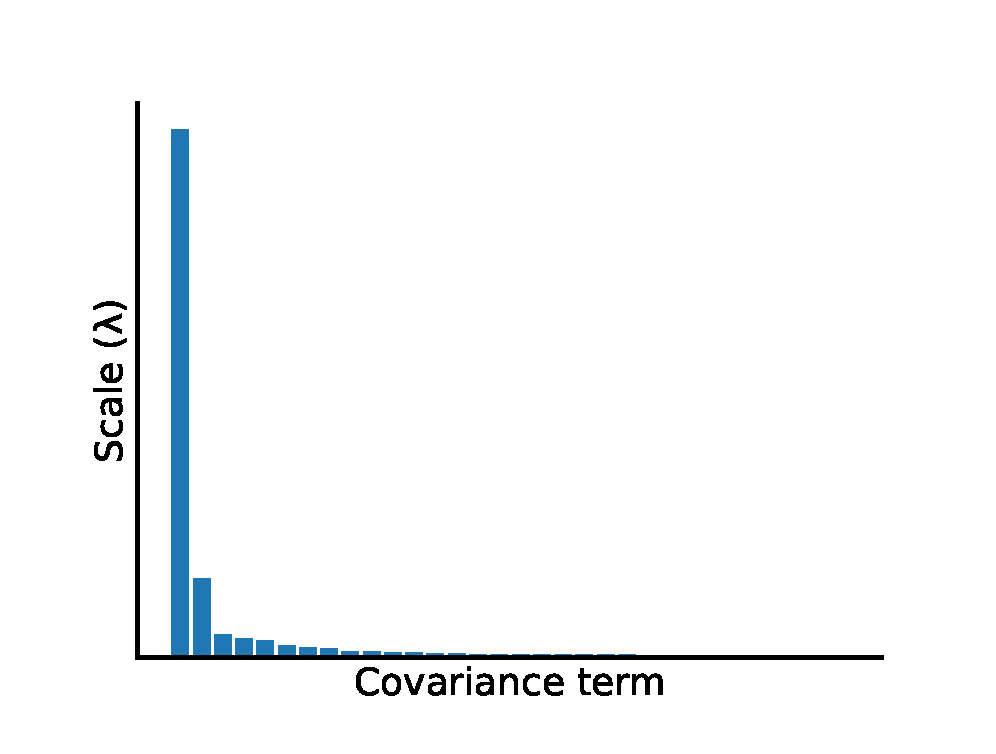
\includegraphics[width=.7\linewidth]{figures/term_relevance.eps}
	\end{minipage}
}

% ================================================================================
\frame{
	\frametitle{Inverse covariance can be calculated quickly}
	\begin{minipage}{.5\linewidth}
		\begin{align*}
			\left(\vcenter{\hbox{\includegraphics[width=.25\linewidth]{figures/sp_cov_2.png}}}\right.
			 & \otimes
			\left.\vcenter{\hbox{\includegraphics[width=.25\linewidth]{figures/tmp_cov_2.png}}}\right)^{-1}
			\\
			=
			\vcenter{\hbox{\includegraphics[width=.25\linewidth]{figures/sp_cov_2.png}}}^{-1}
			 & \otimes
			\vcenter{\hbox{\includegraphics[width=.25\linewidth]{figures/tmp_cov_2.png}}}^{-1} \\
			=
			\vcenter{\hbox{\includegraphics[width=.25\linewidth]{figures/sp_prec_3.png}}}
			 & \otimes
			\vcenter{\hbox{\includegraphics[width=.25\linewidth]{figures/tmp_prec_3.png}}}
		\end{align*}
	\end{minipage}%
	\begin{minipage}{.5\linewidth}
		\includegraphics[width=\linewidth]{figures/struct_prec.png}
	\end{minipage}
}

\frame{
	\frametitle{Structured MDA is more accurate and lightweight}
	\begin{minipage}[b]{.5\linewidth}
		\includegraphics[width=\linewidth]{figures/accuracy.eps}
	\end{minipage}%
	\begin{minipage}[b]{.5\linewidth}
		\includegraphics[width=\linewidth]{figures/training_time.eps}
	\end{minipage}
}
\frame{
	\frametitle{Structured covariance estimation \\
		exploits prior knowledge to:}
	\begin{changemargin}
		\begin{itemize}
			\item Decrease training time \smallskip
			\item Decrease memory usage \smallskip
			\item Decrease calibration time
		\end{itemize}
		\bigskip
	\end{changemargin}
	\bigskip
	\bigskip

	By reducing the number of parameters.
}

% ================================================================================
\frame{
	\begin{changemargin}
		\includegraphics[width=\linewidth]{images/logo.png}
	\end{changemargin}

	\bigskip
	Arne Van Den Kerchove, Arno Libert, Benjamin Wittevrongel,
	Marc M. Van Hulle. Classification of Event-Related Potentials
	with Regularized Spatiotemporal LCMV Beamforming.
	\textit{Applied Sciences}. 2022;

}
\frame{
$$
	\tilde{S}_{k+1} =
	\frac{1}{n}
	\sum^n_{i=1}X_i^\intercal\hat{T}_k^+X_i
$$
$$
	\tilde{T}_{k+1} =
	\frac{1}{n}
	\sum^n_{i=1}X_i\hat{S}_k^+X_i^\intercal
$$
$$
	\tilde{S}_{k+1}^{(\beta)} =
	(1-\beta_{k+1})\tilde{S}_{k+1}
	+\beta_{k+1}\frac{\text{Tr}(\tilde{S}_{k+1})}{c}\mathbb{I}
$$
$$
	\tilde{T}_{k+1}^{(\gamma)} =
	(1-\gamma_{k+1})\tilde{T}_{k+1}
	+\gamma_{k+1}\frac{\text{Tr}(\tilde{T}_{k+1})}{s}\mathbb{I}
$$
$$
	\hat{S}_{k+1} =
	\frac{c}{\text{Tr}\left[\tilde{S}_{k+1}^{(\beta)}\right]}
	\tilde{S}_{k+1}^{(\beta)}
$$
$$
	\hat{T}_{k+1} =
	\frac{s}{\text{Tr}\left[\tilde{T}_{k+1}^{(\gamma)}\right]}
	\tilde{T}_{k+1}^{(\gamma)}
$$

}
\end{document}
